\chapter{Instruction Set Principles}

\section{Introduzione all'Instruction Set Architecture (ISA)}
L'\textbf{Instruction Set Architecture (ISA)} rappresenta l'interfaccia tra l'hardware e il software; è il modo in cui il calcolatore viene visto dal programmatore o dal compilatore. 
Il progettista di un'architettura ha a disposizione molte alternative, e ogni scelta modifica il modo in cui le istruzioni vengono codificate. 

Le diverse alternative vengono valutate in base a:
\begin{itemize}
    \item Prestazioni del processore (Processor performance);
    \item Complessità del processore (Processor complexity);
    \item Complessità del compilatore (Compiler complexity);
    \item Dimensione del codice generato (Code size);
    \item Consumo di potenza (Power consumption).
\end{itemize}

\begin{remark}
La scelta dell'ISA è critica. Ad esempio, oggi molti processori per laptop (come gli Intel 8086 e successivi) si presentano all'esterno come architetture CISC (Complex Instruction Set Computer) con istruzioni molto complesse, ma internamente decodificano queste istruzioni in micro-operazioni tipiche di un'architettura RISC (Reduced Instruction Set Computer) per ottimizzare le prestazioni.
\end{remark}

\section{Modelli di Memorizzazione Interna}
Una delle prime scelte architetturali riguarda dove salvare i dati che il processore andrà a elaborare. Esistono diverse opzioni storiche e attuali:

\begin{enumerate}
    \item \textbf{Stack}: I dati sono salvati in una struttura a pila gestita dal \textit{Top of Stack (TOS)}. Le operazioni aritmetiche non specificano gli operandi, ma utilizzano implicitamente i primi elementi dello stack.
    \item \textbf{Accumulatore}: Utilizzato in architetture storiche (e oggi in moduli di accelerazione AI come i MAC - Multiply and Accumulate). L'accumulatore funge sempre da operando implicito e da registro di destinazione.
    \item \textbf{Registro - Memoria (CISC)}: Le operazioni possono avvenire combinando un dato presente in un registro e uno presente direttamente in memoria (es. architetture 80x86).
    \item \textbf{Registro - Registro / Load-Store (RISC)}: Tutte le operazioni aritmetico-logiche avvengono esclusivamente tra registri interni. Per elaborare un dato in memoria, esso deve essere prima caricato in un registro tramite un'istruzione indipendente. (Es. RISC-V, ARM, MIPS).
\end{enumerate}

\begin{example}
Consideriamo l'operazione di alto livello \( C = A + B \). Vediamo come viene tradotta nei diversi modelli:
\begin{itemize}
    \item \textbf{Stack}: \texttt{push A}, \texttt{push B}, \texttt{add}, \texttt{pop C}. (L'istruzione \texttt{add} sa già dove prendere i dati).
    \item \textbf{Accumulatore}: \texttt{load A}, \texttt{add B}, \texttt{store C}. (\texttt{add} somma B al valore già in accumulatore).
    \item \textbf{Registro-Memoria}: \texttt{load R1, A}, \texttt{add R1, B}, \texttt{store R1, C}.
    \item \textbf{Registro-Registro (Load-Store)}: \texttt{load R1, A}, \texttt{load R2, B}, \texttt{add R3, R1, R2}, \texttt{store R3, C}. 
\end{itemize}
Nonostante l'approccio Load-Store richieda più istruzioni, le singole istruzioni sono molto più semplici, permettendo di abbassare il consumo di potenza e aumentare le prestazioni riducendo il tempo di ciclo (eseguendo idealmente un'istruzione per ciclo di clock).
\end{example}

\section{Organizzazione della Memoria e Accesso ai Dati}
L'accesso alla memoria solleva il problema di come i dati (composti da più byte) vengano salvati.
Esistono due convenzioni principali:
\begin{itemize}
    \item \textbf{Little Endian}: Il byte meno significativo del dato si trova all'indirizzo più basso. (Convenzione che useremo maggiormente).
    \item \textbf{Big Endian}: Il byte più significativo si trova all'indirizzo più basso.
\end{itemize}
Il processore e la memoria devono condividere la stessa convenzione, altrimenti i valori letti saranno errati. 

\section{Modi di Indirizzamento (Addressing Modes)}
I modi di indirizzamento definiscono come il processore calcola l'\textit{Effective Address} (indirizzo effettivo) per accedere ai dati. Sperimentalmente, \textbf{Displacement, Immediato e Registro Indiretto} coprono dal 75\% al 99\% dei casi d'uso nei benchmark.

\begin{itemize}
    \item \textbf{Register mode} (\texttt{Add R4, R3}): Nessun accesso a memoria. Il dato è già nel banco dei registri (General Purpose Registers). Altamente utilizzato.
    \item \textbf{Immediate mode} (\texttt{Add R4, \#3}): Il dato è una costante definita direttamente all'interno dell'istruzione. Analisi empiriche mostrano che 8-16 bit sono sufficienti per rappresentare il 50-80\% dei valori immediati necessari.
    \item \textbf{Displacement mode} (\texttt{Add R4, 100(R1)}): L'indirizzo effettivo è la somma di una costante (es. 100) e il valore contenuto in un registro base (R1). Molto utile per accedere a variabili locali o campi di struct. Solitamente richiede dai 12 ai 16 bit nell'istruzione.
    \item \textbf{Register Deferred / Indirect} (\texttt{Add R4, (R1)}): Il registro contiene l'indirizzo di memoria del dato (funge da puntatore).
    \item \textbf{Indexed / Scaled / Auto-increment}: Modi più complessi (molto usati nei CISC, quasi assenti nei RISC per mantenere semplice l'hardware). Ad esempio l'Auto-incremento è utile per scorrere i vettori, mentre lo Scaled mode moltiplica il valore dell'indice per la dimensione del dato (es. 1, 4, 8 byte).
\end{itemize}

\section{Operazioni nell'Instruction Set e Frequenze d'Uso}
Le istruzioni si dividono in categorie logiche:
\begin{table}[H]
\centering
\begin{tabular}{|l|p{10cm}|}
\hline
\textbf{Tipo di Operatore} & \textbf{Esempi} \\ \hline
Aritmetiche e Logiche & Add, And, Subtract, Or \\ \hline
Trasferimento Dati & Load, Store (su macchine con memory addressing) \\ \hline
Controllo & Branch (salti condizionati), Jump (salti incondizionati), Call, Return \\ \hline
Sistema & System call, gestione memoria virtuale \\ \hline
Virgola Mobile (Floating Point) & Add FP, Multiply FP \\ \hline
\end{tabular}
\caption{Classificazione delle istruzioni.}
\end{table}

Analizzando i benchmark reali (es. SPECint2006 per RISC-V e programmi interi per 80x86):
\begin{itemize}
    \item Nelle architetture CISC (80x86) storiche si cercava di ottimizzare le istruzioni più frequenti (Load 22\%, Branch 20\%, Compare 16\%, Store 12\%).
    \item Nelle architetture RISC (come RISC-V), le operazioni \textbf{ALU dominano (circa 42\%)} seguite da \textbf{Load (24\%)}, \textbf{Branches (17\%)} e \textbf{Stores (11\%)}. L'obiettivo dei RISC non è ottimizzare un'istruzione specifica, ma garantire che \textit{tutte} impieghino lo stesso tempo di esecuzione.
\end{itemize}

\section{Istruzioni di Controllo del Flusso (Control Flow)}
Le istruzioni di controllo del flusso modificano il Program Counter (PC) e si dividono in: salti condizionati (\textit{conditional branches}), salti incondizionati (\textit{jumps}), chiamate a procedura (\textit{procedure calls}) e ritorni (\textit{returns}).

\subsection{L'indirizzo di Destinazione (Destination Address)}
Normalmente, per i salti condizionati, l'indirizzo di destinazione viene specificato come un \textbf{displacement rispetto al valore corrente del Program Counter (PC-Relative)}.
\begin{remark}
Usare un indirizzamento relativo al PC (es. PC + offset) è fondamentale perché permette di generare codice \textit{Position Independent} (indipendente dalla posizione di memoria in cui il programma viene caricato). Evita l'uso di indirizzi assoluti che vincolerebbero il programma a una specifica zona di memoria.
\end{remark}

\subsection{Salti a Registro (Register Indirect Jumps) e Procedure}
Per distanze molto grandi, o per indirizzi non noti a tempo di compilazione, si carica l'indirizzo target in un registro e si esegue un salto indiretto.
Questo permette di:
\begin{itemize}
    \item Implementare costrutti come \texttt{switch} / \texttt{case} in C;
    \item Supportare librerie dinamiche condivise (.dll, .so);
    \item Supportare le funzioni virtuali (Object-Oriented Programming).
\end{itemize}

\subsection{Valutazione delle Condizioni}
I salti condizionati (di gran lunga i più eseguiti, in particolare le comparazioni "Minore di" e "Uguale a", che coprono il 70\% dei casi) possono essere implementati in vari modi a seconda dell'architettura:

\begin{table}[H]
\centering
\begin{tabular}{|p{3cm}|p{3cm}|p{8cm}|}
\hline
\textbf{Metodo} & \textbf{Esempi} & \textbf{Caratteristiche} \\ \hline
\textbf{Condition Code (CC)} & 80x86, ARM & L'ALU setta automaticamente dei flag (Zero, Carry, Negative). Vantaggio: a volte la condizione è "gratis". Svantaggio: il CC è uno stato extra, crea dipendenze tra l'istruzione aritmetica e il salto. (In ARM i CC possono rendere \textit{ogni} istruzione condizionale). \\ \hline
\textbf{Condition Register} & MIPS, Alpha & Testa un registro arbitrario in seguito a un confronto (es. se uguale a zero). Semplice, ma può richiedere confronti extra. \\ \hline
\textbf{Compare and Branch} & RISC-V, PA-RISC & La comparazione (es. "maggiore", "minore") è inclusa direttamente nell'istruzione di salto. Vantaggio: 1 istruzione invece di 2. Svantaggio: può creare percorsi critici lunghi (critical paths) nell'hardware del processore. \\ \hline
\end{tabular}
\caption{Valutazione delle condizioni nei rami di esecuzione.}
\end{table}

\subsection{Gestione delle Procedure (Procedure Calls)}
Quando si chiama una procedura, è necessario salvare due tipi di informazioni:
\begin{enumerate}
    \item \textbf{Return Address}: L'indirizzo a cui ritornare (tipicamente salvato in un registro dedicato).
    \item \textbf{Registri acceduti}: Devono essere preservati. Esistono due convenzioni:
    \begin{itemize}
        \item \textit{Caller saving}: Il chiamante salva i registri prima di invocare la procedura.
        \item \textit{Callee saving}: La procedura invocata salva i registri che intende "sporcare" e li ripristina prima del return.
    \end{itemize}
\end{enumerate}

\section{Tipi e Dimensioni degli Operandi}
La dimensione minima indirizzabile è tipicamente il \textit{Byte} (8 bit). Le tipologie supportate solitamente includono:
\begin{itemize}
    \item Char (1 byte)
    \item Half word (2 byte)
    \item Word (4 byte - standard per interi a 32 bit, copre il 74\% degli accessi per programmi interi)
    \item Double word (8 byte - molto usata per i numeri reali Double Precision)
    \item Floating-point singola e doppia precisione (4 e 8 byte).
\end{itemize}

% FIGURA DA INSERIRE QUI
% Fonte: Slide 39
% Descrizione: Grafico a barre che mostra la distribuzione degli accessi in memoria in base alla dimensione del dato (Byte, Half Word, Word, Double Word) separato per programmi Interi e Floating-Point.
\begin{figure}[H]
    \centering
    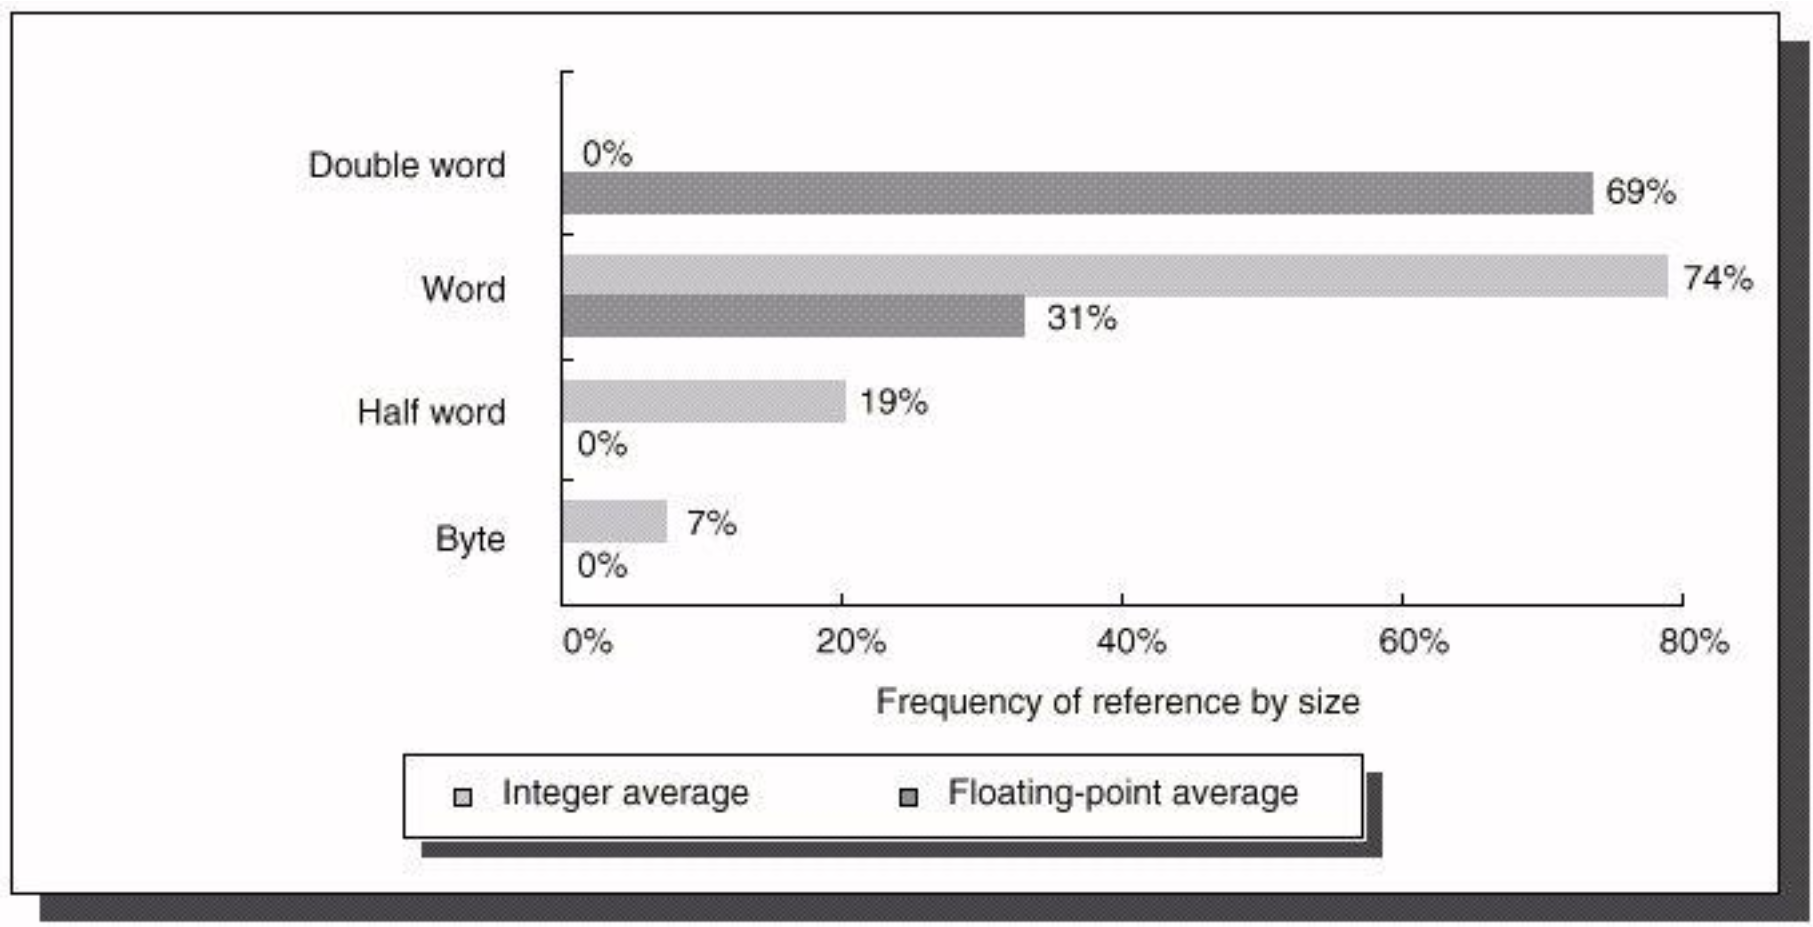
\includegraphics[width=0.8\textwidth]{capitoli/02_intro_to_instruction-set/images/data.png}
    \caption{Distribuzione degli accessi ai dati per dimensione.}
    \label{fig:data_access_size}
\end{figure}

\section{Codifica dell'Instruction Set (Instruction Set Encoding)}
Come vengono codificate le istruzioni (Opcode, registri, costanti) nei bit a disposizione (es. 32 bit)? Dipende da quante istruzioni e da quanti modi di indirizzamento esistono.
Esistono tre filosofie principali:

\subsection{Codifica Variabile (Es. Intel 80x86, VAX)}
\begin{itemize}
    \item La lunghezza dell'istruzione varia (da 1 a molti byte).
    \item Può supportare un numero qualsiasi di operandi e include specificatori di indirizzamento direttamente accanto all'operando.
    \item \textbf{Vantaggio}: Dimensione del codice generato (Code size) minima.
    \item \textbf{Svantaggio}: Prestazioni ridotte, decodifica hardware estremamente complessa (il calcolo del PC successivo dipende dalla comprensione immediata della lunghezza dell'istruzione corrente).
\end{itemize}

\subsection{Codifica Fissa (Es. RISC-V, ARM, MIPS)}
\begin{itemize}
    \item La lunghezza dell'istruzione è sempre fissa (tipicamente 32 bit).
    \item Numero fisso di operandi (sempre 3 per le operazioni ALU) e campi fissi.
    \item \textbf{Vantaggio}: Massime prestazioni e facilità di progettazione del datapath (il calcolo del PC successivo è semplicemente \texttt{PC + 4}).
    \item \textbf{Svantaggio}: Dimensione del codice maggiore (anche istruzioni semplici occupano 32 bit).
\end{itemize}

\subsection{Codifica Ibrida (Es. RISC-V Compressed, ARM Thumb-2)}
\begin{itemize}
    \item Offre formati multipli decisi dall'opcode (es. istruzioni a 16 bit per operazioni molto comuni e 32 bit per il resto).
    \item \textbf{Vantaggio}: Ottimo compromesso (trade-off) tra dimensione del codice compatta e alte prestazioni in fase di decodifica, lasciato spesso alla gestione del compilatore.
\end{itemize}

% FIGURA DA INSERIRE QUI
% Fonte: Slide 44 (che riassume la slide 41, 42, 43)
% Descrizione: Diagramma a blocchi che confronta la struttura della codifica Variabile (A), Fissa (B) e Ibrida (C).
\begin{figure}[H]
    \centering
    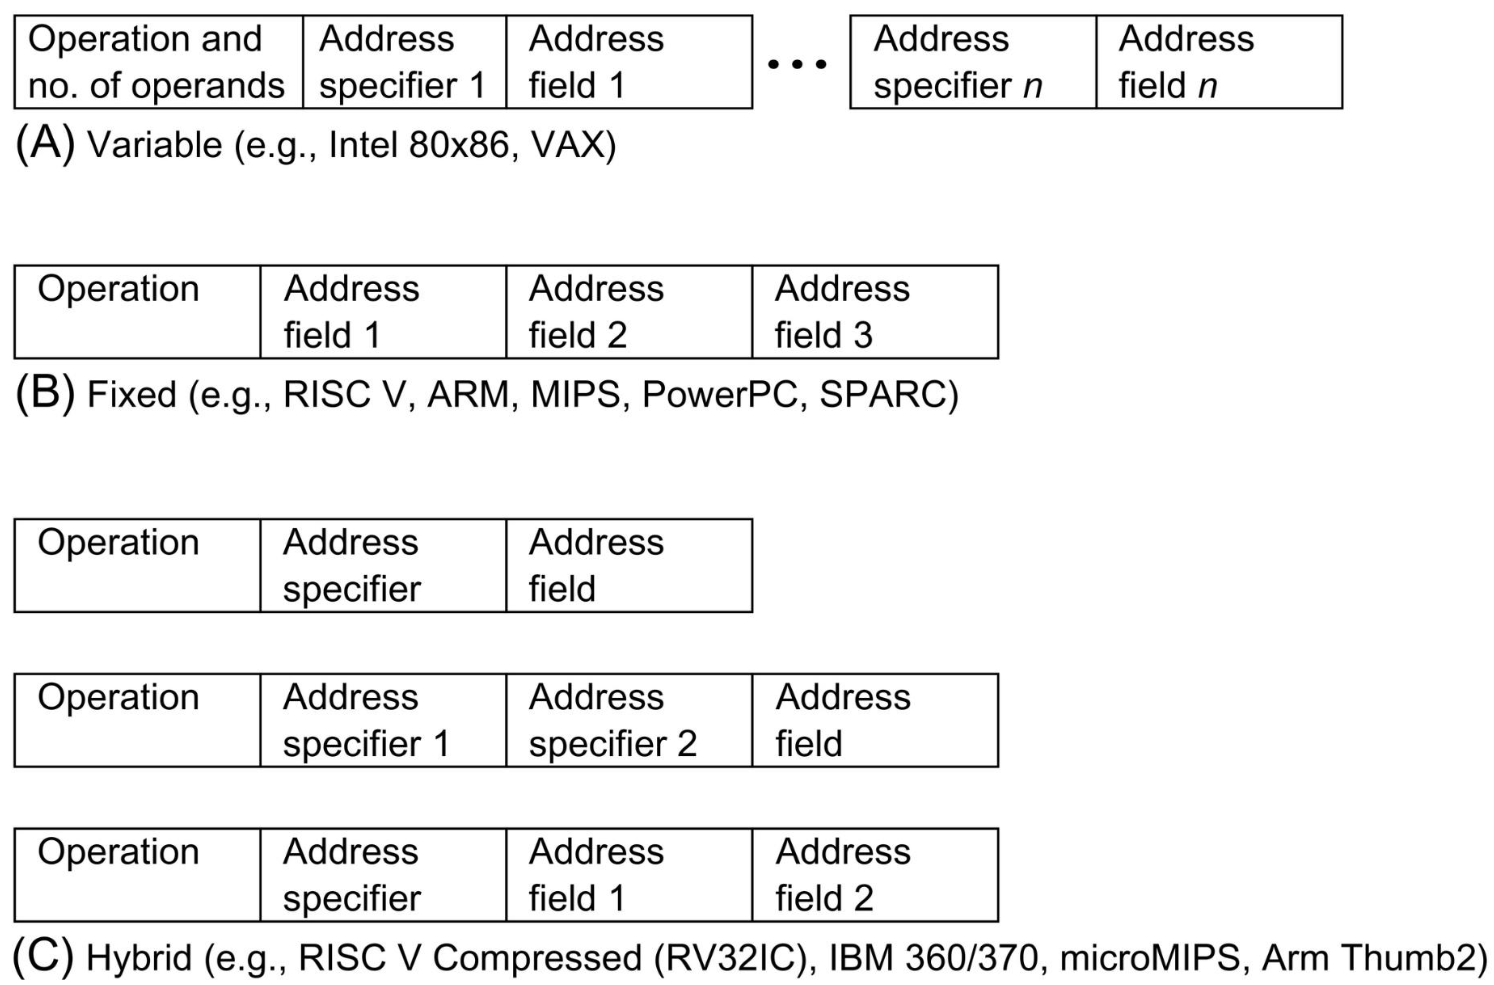
\includegraphics[width=0.9\textwidth]{capitoli/02_intro_to_instruction-set/images/image.png}
    \caption{Confronto tra i modelli di decodifica: Variabile, Fissa e Ibrida.}
    \label{fig:encoding_types}
\end{figure}

\begin{remark}[Conflitti Progettuali (Conflicting Issues)]
Il progettista di ISA affronta un problema di ottimizzazione contrastante: bilanciare la compattezza del codice (\textit{code size}), la ricchezza dell'ISA (numero di registri e modi di indirizzamento) e la semplicità/velocità dell'hardware di \textit{fetch e decodifica}. Architetture moderne tendono verso la semplicità (RISC) affiancando estensioni compresse (Thumb2 / RV32IC) per recuperare compattezza del codice.
\end{remark}